% !TEX root = Master.tex

\autoref{fig:kcc_pair_scatterplots} is hinting that the marginal distributions come with a noticeable skewness, which are best to take into account. Among a pool of possible parametric distributions, we pick an appropriate one for each marginal. Several distributions would theoretically be justifying the shape of our data, e.g. Weibull, Gamma, Fisk (or Log-logistic), Singh-Maddala or Dagum distribution. After screening those parametric distributions, we find that the Dagum distribution fits all three marginals fairly well \citep{dagum1975model}. Although the distribution assumptions are aligned with the empirical distributions of the data, there are still some expected outliers. This is quite visible in Figures \ref{fig:kcc_2_marginal} - \ref{fig:kcc_8_marginal}, which depict the marginal empirical distributions along with the theoretical assumptions, especially when looking at the Quantile-Quantile Plots (right figures).



 \begin{figure}[H]
\centering
\begin{subfigure}{.45\textwidth}
  \centering
  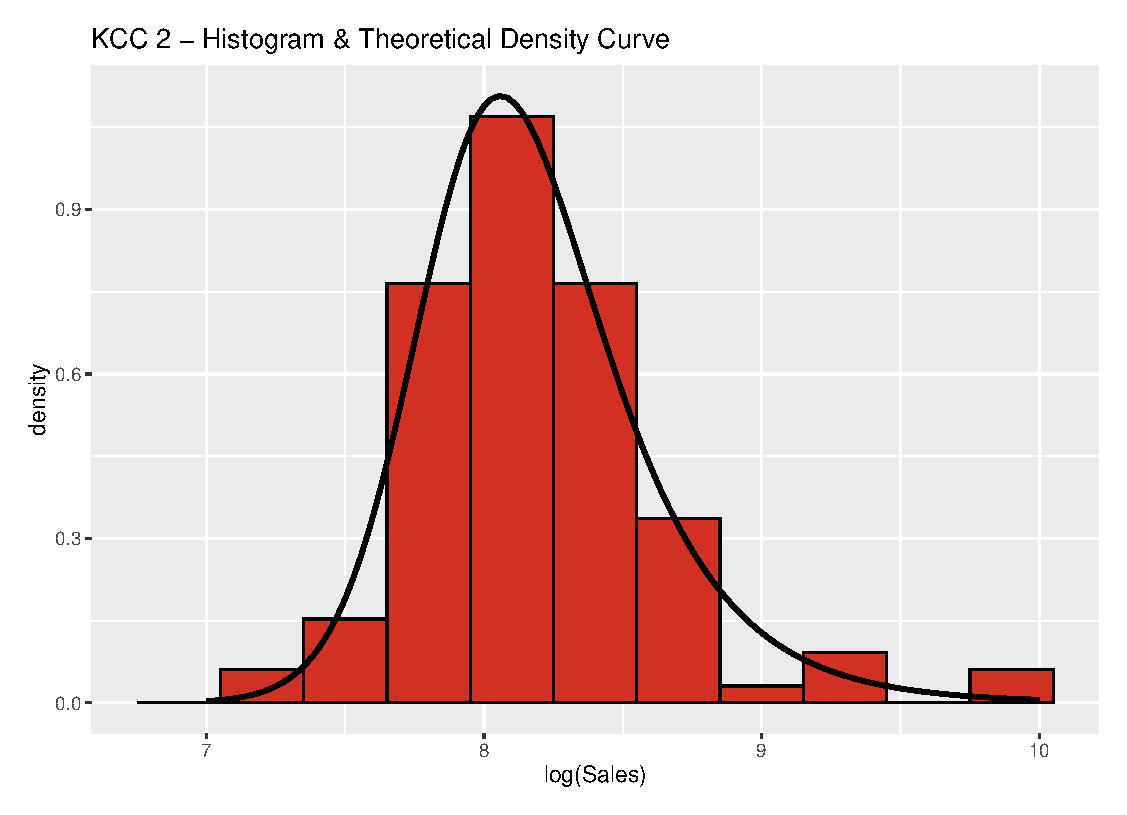
\includegraphics[width=\linewidth]{figures/kcc_2_density.eps}
  \caption{Histogram \& theoretical density}
  \label{fig:kcc_2_density}
\end{subfigure}
\begin{subfigure}{.45\textwidth}
  \centering
  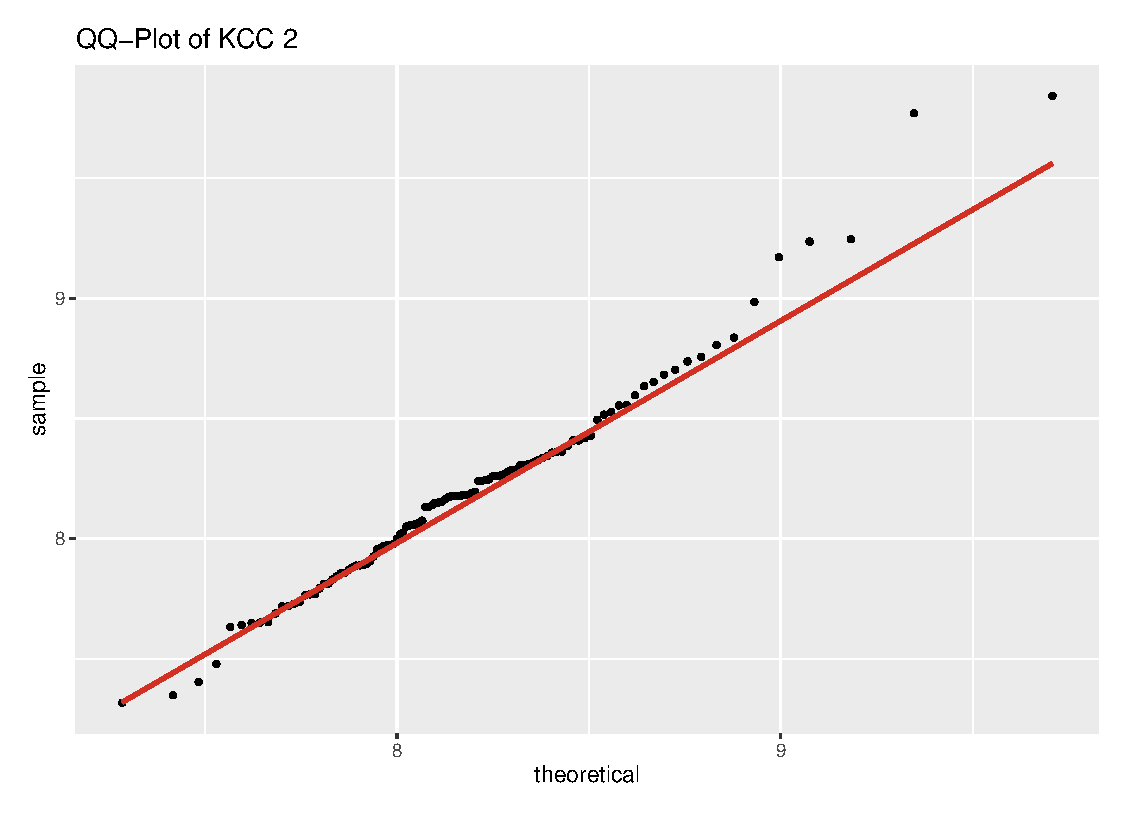
\includegraphics[width=\linewidth]{figures/kcc_2_qqplot.eps}
  \caption{QQ-Plot}
  \label{fig:kcc_2_qqplot}
\end{subfigure}
\caption{Dagum distribution fitted to log-sales of \ac{KCC} 2; Estimated parameters: scale = 7.83, shape1.a = 29.15, shape2.p = 2.42}
\label{fig:kcc_2_marginal}
\end{figure} 





\begin{figure}[H]
\centering
\begin{subfigure}{.45\textwidth}
  \centering
  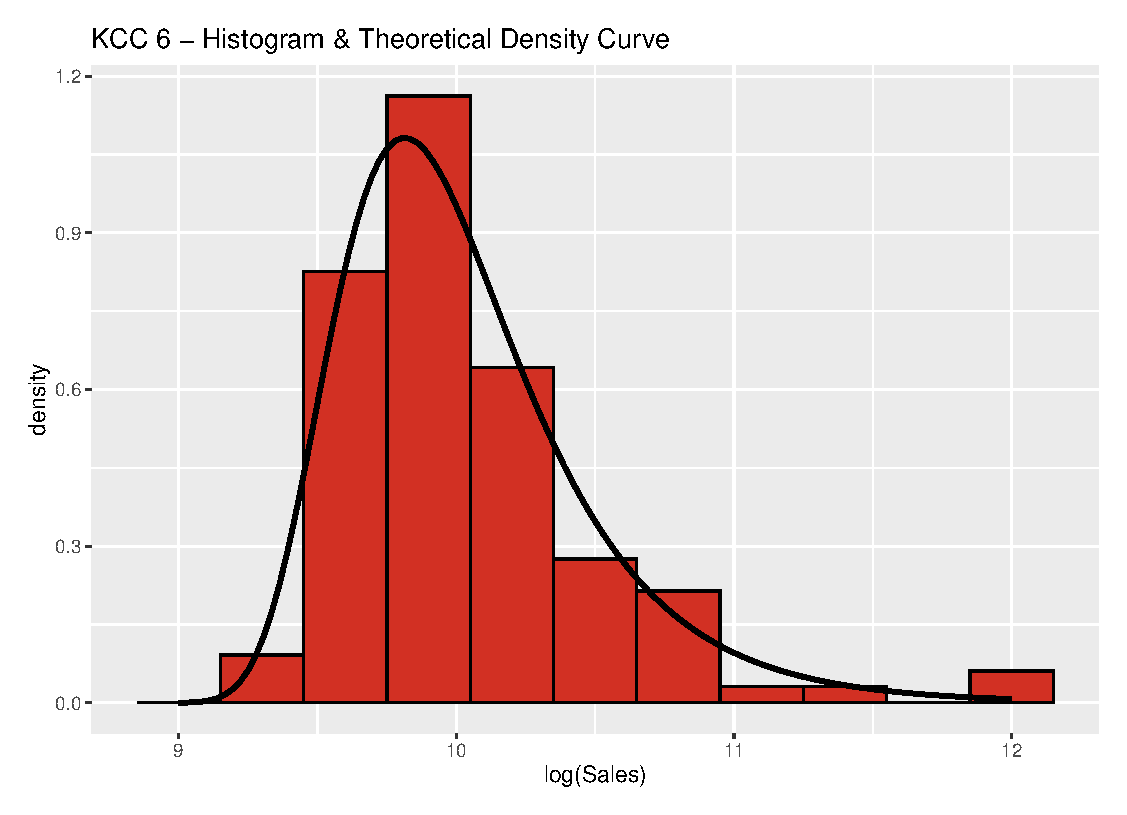
\includegraphics[width=\linewidth]{figures/kcc_6_density.eps}
  \caption{Histogram \& theoretical density}
  \label{fig:kcc_6_density}
\end{subfigure}
\begin{subfigure}{.45\textwidth}
  \centering
  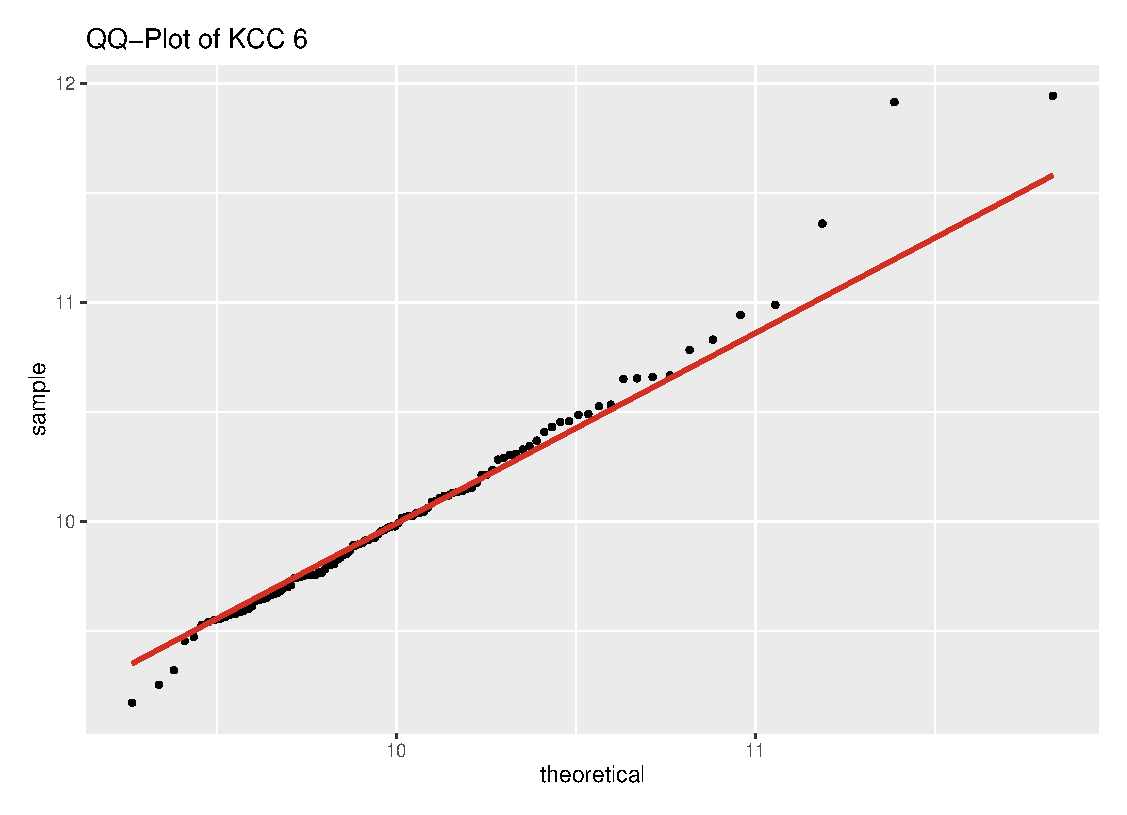
\includegraphics[width=\linewidth]{figures/kcc_6_qqplot.eps}
  \caption{QQ-Plot}
  \label{fig:kcc_6_qqplot}
\end{subfigure}
\caption{Dagum distribution fitted to log-sales of \ac{KCC} 6; Estimated parameters: scale = 8.32, shape1.a = 29, shape2.p = 122.95}
\label{fig:kcc_6_marginal}
\end{figure} 




\begin{figure}[H]
\centering
\begin{subfigure}{.45\textwidth}
  \centering
  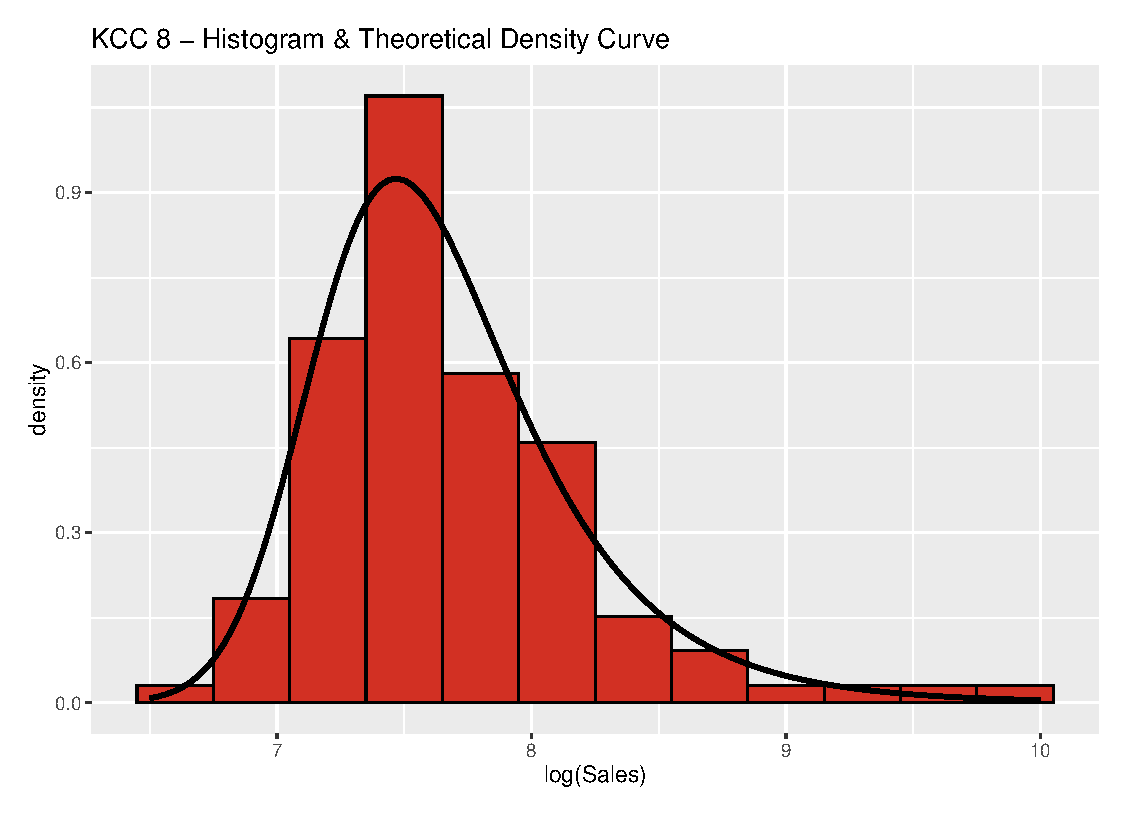
\includegraphics[width=\linewidth]{figures/kcc_8_density.eps}
  \caption{Histogram \& theoretical density}
  \label{fig:kcc_8_density}
\end{subfigure}
\begin{subfigure}{.45\textwidth}
  \centering
  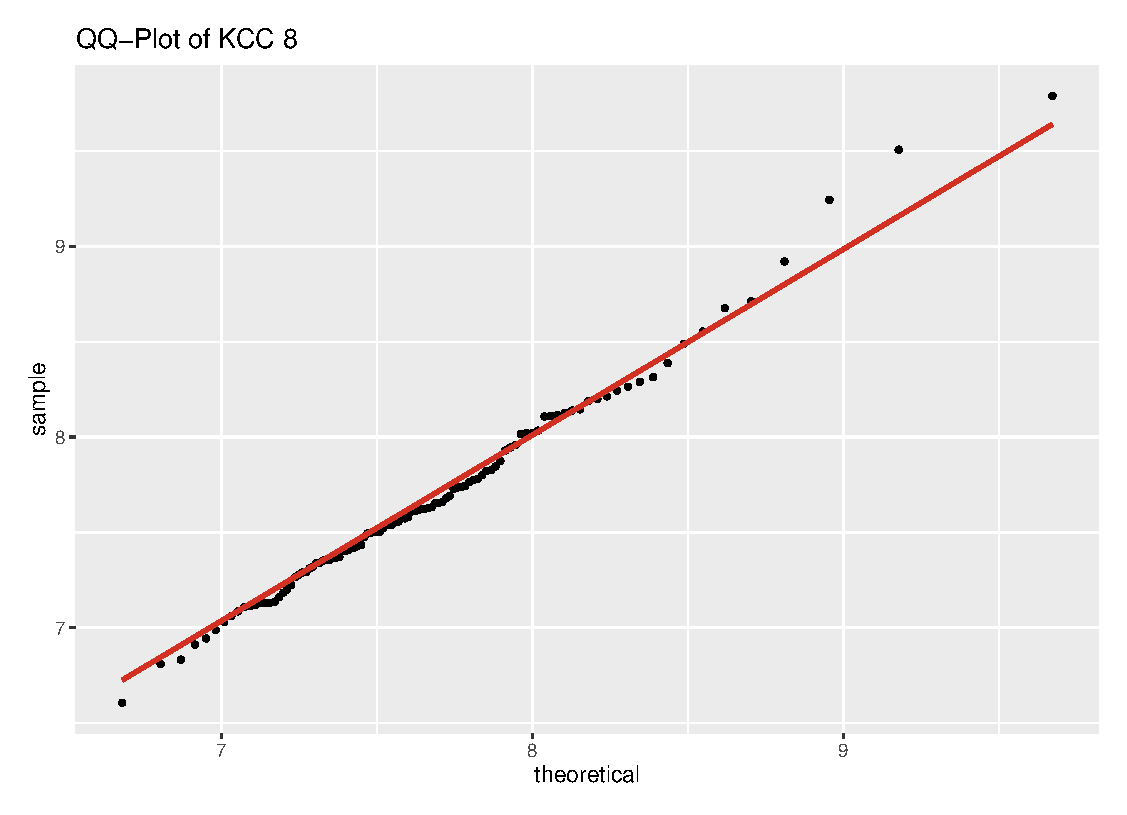
\includegraphics[width=\linewidth]{figures/kcc_8_qqplot.eps}
  \caption{QQ-Plot}
  \label{fig:kcc_8_qqplot}
\end{subfigure}
\caption{Dagum distribution fitted to log-sales of \ac{KCC} 8; Estimated parameters: scale = 7, shape1.a = 21.03, shape2.p = 4.13}
\label{fig:kcc_8_marginal}
\end{figure} 


For the approaches in the below Section \ref{ssec:kcc_correlations} requiring parametric distribution assumptions for the marginals, we will consider the Dagum distribution with parameters specified as in the captions of the above three figures, which represent estimated maximum likelihood values (that is, if they do not have to be estimated over again within a model like e.g. \ac{GAMLSS}).



